\documentclass{standalone}
\usepackage{tikz}
\usetikzlibrary{patterns, positioning}


\begin{document}
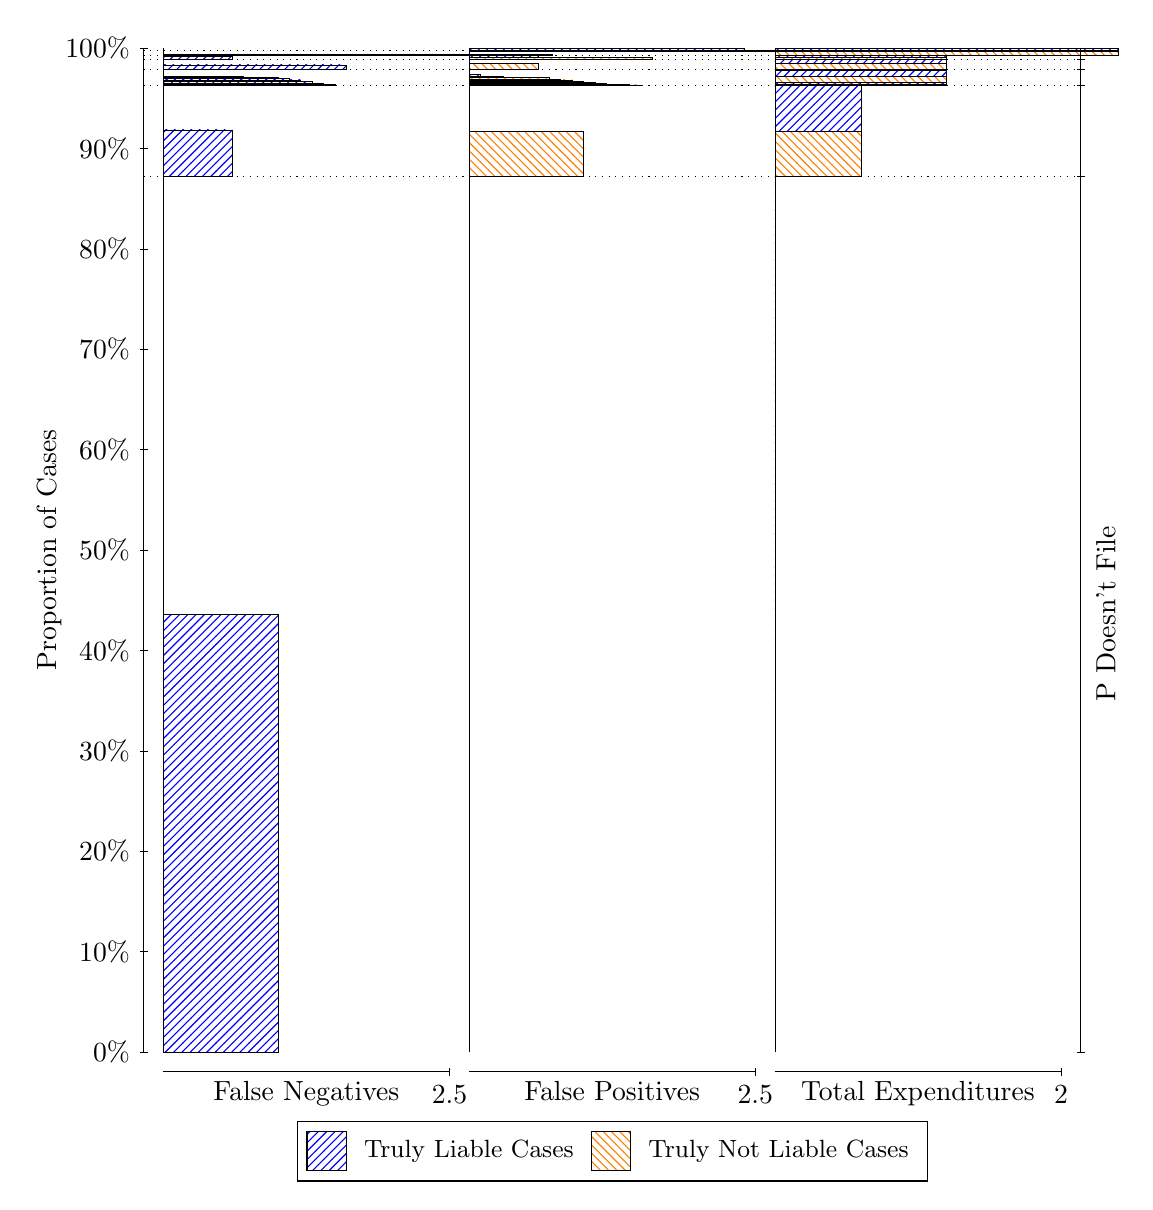
\begin{tikzpicture}
\draw[black, very thin] (1.5,1.75) -- (1.5,14.5);
\node[rotate=90, text=black, anchor=center] at (0.3, 8.125) {Proportion of Cases};
\draw[black, very thin] (1.45,1.75) -- (1.55,1.75);
\node[text=black, anchor=east] at (1.45, 1.75) {0\%};
\draw[black, very thin] (1.45,3.025) -- (1.55,3.025);
\node[text=black, anchor=east] at (1.45, 3.025) {10\%};
\draw[black, very thin] (1.45,4.3) -- (1.55,4.3);
\node[text=black, anchor=east] at (1.45, 4.3) {20\%};
\draw[black, very thin] (1.45,5.575) -- (1.55,5.575);
\node[text=black, anchor=east] at (1.45, 5.575) {30\%};
\draw[black, very thin] (1.45,6.85) -- (1.55,6.85);
\node[text=black, anchor=east] at (1.45, 6.85) {40\%};
\draw[black, very thin] (1.45,8.125) -- (1.55,8.125);
\node[text=black, anchor=east] at (1.45, 8.125) {50\%};
\draw[black, very thin] (1.45,9.4) -- (1.55,9.4);
\node[text=black, anchor=east] at (1.45, 9.4) {60\%};
\draw[black, very thin] (1.45,10.675) -- (1.55,10.675);
\node[text=black, anchor=east] at (1.45, 10.675) {70\%};
\draw[black, very thin] (1.45,11.95) -- (1.55,11.95);
\node[text=black, anchor=east] at (1.45, 11.95) {80\%};
\draw[black, very thin] (1.45,13.225) -- (1.55,13.225);
\node[text=black, anchor=east] at (1.45, 13.225) {90\%};
\draw[black, very thin] (1.45,14.5) -- (1.55,14.5);
\node[text=black, anchor=east] at (1.45, 14.5) {100\%};

\draw[black, very thin] (13.4,1.75) -- (13.4,14.5);
\draw[black, very thin] (13.35,1.75) -- (13.45,1.75);
\node[anchor=west] at (13.35, 1.75) {};
\draw[black, very thin] (13.35,12.874) -- (13.45,12.874);
\node[anchor=west] at (13.35, 12.874) {};
\draw[black, very thin] (13.35,14.028) -- (13.45,14.028);
\node[anchor=west] at (13.35, 14.028) {};
\draw[black, very thin] (13.35,14.232) -- (13.45,14.232);
\node[anchor=west] at (13.35, 14.232) {};
\draw[black, very thin] (13.35,14.358) -- (13.45,14.358);
\node[anchor=west] at (13.35, 14.358) {};
\draw[black, very thin] (13.35,14.409) -- (13.45,14.409);
\node[anchor=west] at (13.35, 14.409) {};
\draw[black, very thin] (13.35,14.464) -- (13.45,14.464);
\node[anchor=west] at (13.35, 14.464) {};
\draw[black, very thin] (13.35,14.5) -- (13.45,14.5);
\node[anchor=west] at (13.35, 14.5) {};

\draw[black, very thin, pattern color=blue, pattern=north east lines] (1.75,1.75) rectangle (3.2033,7.3121);
\draw[black, very thin, pattern color=orange, pattern=north west lines] (1.75,7.3121) rectangle (1.75,12.874);
\draw[black, very thin, pattern color=blue, pattern=north east lines] (1.75,12.874) rectangle (2.622,13.461);
\draw[black, very thin, pattern color=orange, pattern=north west lines] (1.75,13.461) rectangle (1.75,14.028);
\draw[black, very thin, pattern color=blue, pattern=north east lines] (1.75,14.028) rectangle (3.93,14.043);
\draw[black, very thin, pattern color=blue, pattern=north east lines] (1.75,14.043) rectangle (3.7847,14.049);
\draw[black, very thin, pattern color=blue, pattern=north east lines] (1.75,14.049) rectangle (3.6393,14.072);
\draw[black, very thin, pattern color=blue, pattern=north east lines] (1.75,14.072) rectangle (3.494,14.094);
\draw[black, very thin, pattern color=blue, pattern=north east lines] (1.75,14.094) rectangle (3.3487,14.117);
\draw[black, very thin, pattern color=blue, pattern=north east lines] (1.75,14.117) rectangle (3.2033,14.124);
\draw[black, very thin, pattern color=blue, pattern=north east lines] (1.75,14.124) rectangle (3.058,14.13);
\draw[black, very thin, pattern color=blue, pattern=north east lines] (1.75,14.13) rectangle (2.9127,14.132);
\draw[black, very thin, pattern color=blue, pattern=north east lines] (1.75,14.132) rectangle (2.7673,14.135);
\draw[black, very thin, pattern color=orange, pattern=north west lines] (1.75,14.135) rectangle (1.75,14.232);
\draw[black, very thin, pattern color=blue, pattern=north east lines] (1.75,14.232) rectangle (4.0753,14.285);
\draw[black, very thin, pattern color=orange, pattern=north west lines] (1.75,14.285) rectangle (1.75,14.358);
\draw[black, very thin, pattern color=blue, pattern=north east lines] (1.75,14.358) rectangle (2.622,14.389);
\draw[black, very thin, pattern color=orange, pattern=north west lines] (1.75,14.389) rectangle (1.75,14.409);
\draw[black, very thin, pattern color=blue, pattern=north east lines] (1.75,14.409) rectangle (6.6913,14.417);
\draw[black, very thin, pattern color=orange, pattern=north west lines] (1.75,14.417) rectangle (1.75,14.464);
\draw[black, very thin, pattern color=orange, pattern=north west lines] (1.75,14.464) rectangle (1.75,14.472);
\draw[black, very thin, pattern color=blue, pattern=north east lines] (1.75,14.472) rectangle (1.75,14.5);
\draw[black, very thin, pattern color=orange, pattern=north west lines] (5.6333,1.75) rectangle (5.6333,7.3122);
\draw[black, very thin, pattern color=blue, pattern=north east lines] (5.6333,7.3122) rectangle (5.6333,12.874);
\draw[black, very thin, pattern color=orange, pattern=north west lines] (5.6333,12.874) rectangle (7.0867,13.442);
\draw[black, very thin, pattern color=blue, pattern=north east lines] (5.6333,13.442) rectangle (5.6333,14.028);
\draw[black, very thin, pattern color=orange, pattern=north west lines] (5.6333,14.028) rectangle (7.8133,14.031);
\draw[black, very thin, pattern color=orange, pattern=north west lines] (5.6333,14.031) rectangle (7.668,14.034);
\draw[black, very thin, pattern color=orange, pattern=north west lines] (5.6333,14.034) rectangle (7.5227,14.039);
\draw[black, very thin, pattern color=orange, pattern=north west lines] (5.6333,14.039) rectangle (7.3773,14.046);
\draw[black, very thin, pattern color=orange, pattern=north west lines] (5.6333,14.046) rectangle (7.232,14.063);
\draw[black, very thin, pattern color=orange, pattern=north west lines] (5.6333,14.063) rectangle (7.0867,14.078);
\draw[black, very thin, pattern color=orange, pattern=north west lines] (5.6333,14.078) rectangle (6.9413,14.096);
\draw[black, very thin, pattern color=orange, pattern=north west lines] (5.6333,14.096) rectangle (6.796,14.103);
\draw[black, very thin, pattern color=orange, pattern=north west lines] (5.6333,14.103) rectangle (6.6507,14.125);
\draw[black, very thin, pattern color=blue, pattern=north east lines] (5.6333,14.125) rectangle (6.36,14.128);
\draw[black, very thin, pattern color=blue, pattern=north east lines] (5.6333,14.128) rectangle (6.2147,14.131);
\draw[black, very thin, pattern color=blue, pattern=north east lines] (5.6333,14.131) rectangle (6.0693,14.137);
\draw[black, very thin, pattern color=blue, pattern=north east lines] (5.6333,14.137) rectangle (5.924,14.143);
\draw[black, very thin, pattern color=blue, pattern=north east lines] (5.6333,14.143) rectangle (5.7787,14.167);
\draw[black, very thin, pattern color=blue, pattern=north east lines] (5.6333,14.167) rectangle (5.6333,14.232);
\draw[black, very thin, pattern color=orange, pattern=north west lines] (5.6333,14.232) rectangle (6.5053,14.305);
\draw[black, very thin, pattern color=blue, pattern=north east lines] (5.6333,14.305) rectangle (5.6333,14.358);
\draw[black, very thin, pattern color=orange, pattern=north west lines] (5.6333,14.358) rectangle (7.9587,14.378);
\draw[black, very thin, pattern color=blue, pattern=north east lines] (5.6333,14.378) rectangle (6.5053,14.409);
\draw[black, very thin, pattern color=orange, pattern=north west lines] (5.6333,14.409) rectangle (5.6333,14.456);
\draw[black, very thin, pattern color=blue, pattern=north east lines] (5.6333,14.456) rectangle (5.6333,14.464);
\draw[black, very thin, pattern color=orange, pattern=north west lines] (5.6333,14.464) rectangle (10.575,14.472);
\draw[black, very thin, pattern color=blue, pattern=north east lines] (5.6333,14.472) rectangle (9.1213,14.5);
\draw[black, very thin, pattern color=orange, pattern=north west lines] (9.5167,1.75) rectangle (9.5167,7.3122);
\draw[black, very thin, pattern color=blue, pattern=north east lines] (9.5167,7.3122) rectangle (9.5167,12.874);
\draw[black, very thin, pattern color=orange, pattern=north west lines] (9.5167,12.874) rectangle (10.607,13.442);
\draw[black, very thin, pattern color=blue, pattern=north east lines] (9.5167,13.442) rectangle (10.607,14.028);
\draw[black, very thin, pattern color=orange, pattern=north west lines] (9.5167,14.028) rectangle (11.697,14.045);
\draw[black, very thin, pattern color=blue, pattern=north east lines] (9.5167,14.045) rectangle (11.697,14.068);
\draw[black, very thin, pattern color=orange, pattern=north west lines] (9.5167,14.068) rectangle (11.697,14.14);
\draw[black, very thin, pattern color=blue, pattern=north east lines] (9.5167,14.14) rectangle (11.697,14.215);
\draw[black, very thin, pattern color=orange, pattern=north west lines] (9.5167,14.215) rectangle (11.697,14.223);
\draw[black, very thin, pattern color=blue, pattern=north east lines] (9.5167,14.223) rectangle (11.697,14.232);
\draw[black, very thin, pattern color=orange, pattern=north west lines] (9.5167,14.232) rectangle (11.697,14.305);
\draw[black, very thin, pattern color=blue, pattern=north east lines] (9.5167,14.305) rectangle (11.697,14.358);
\draw[black, very thin, pattern color=orange, pattern=north west lines] (9.5167,14.358) rectangle (11.697,14.378);
\draw[black, very thin, pattern color=blue, pattern=north east lines] (9.5167,14.378) rectangle (11.697,14.409);
\draw[black, very thin, pattern color=orange, pattern=north west lines] (9.5167,14.409) rectangle (13.877,14.456);
\draw[black, very thin, pattern color=blue, pattern=north east lines] (9.5167,14.456) rectangle (13.877,14.464);
\draw[black, very thin, pattern color=orange, pattern=north west lines] (9.5167,14.464) rectangle (13.877,14.472);
\draw[black, very thin, pattern color=blue, pattern=north east lines] (9.5167,14.472) rectangle (13.877,14.5);
\draw[black, dotted] (1.5,12.874) -- (13.4,12.874);
\draw[black, dotted] (1.5,14.028) -- (13.4,14.028);
\draw[black, dotted] (1.5,14.232) -- (13.4,14.232);
\draw[black, dotted] (1.5,14.358) -- (13.4,14.358);
\draw[black, dotted] (1.5,14.409) -- (13.4,14.409);
\draw[black, dotted] (1.5,14.464) -- (13.4,14.464);
\draw[black, very thin] (1.75,1.5) -- (5.3833,1.5);
\node[text=black, anchor=north] at (3.5667, 1.5) {False Negatives};
\draw[black, very thin] (5.3833,1.45) -- (5.3833,1.55);
\node[text=black, anchor=north] at (5.3833, 1.45) {2.5};

\draw[black, very thin] (5.6333,1.5) -- (9.2667,1.5);
\node[text=black, anchor=north] at (7.45, 1.5) {False Positives};
\draw[black, very thin] (9.2667,1.45) -- (9.2667,1.55);
\node[text=black, anchor=north] at (9.2667, 1.45) {2.5};

\draw[black, very thin] (9.5167,1.5) -- (13.15,1.5);
\node[text=black, anchor=north] at (11.333, 1.5) {Total Expenditures};
\draw[black, very thin] (13.15,1.45) -- (13.15,1.55);
\node[text=black, anchor=north] at (13.15, 1.45) {2};

\node[text=black, centered, rotate=90] at (13.72, 7.3121) {P Doesn't File};







\draw (7.449999999999999,1.5) node[draw=none] (baseCoordinate) {};
\begin{scope}[align=center]
        \matrix[scale=0.5, draw=black, below=0.5cm of baseCoordinate, nodes={draw}, column sep=0.1cm]{
            \node[rectangle, draw, minimum width=0.5cm, minimum height=0.5cm, pattern color=blue, pattern=north east lines] {}; &
            \node[draw=none, font=\small, text=black] (B) {Truly Liable Cases}; &
            \node[rectangle, draw, minimum width=0.5cm, minimum height=0.5cm, pattern color=orange, pattern=north west lines] {}; &
            \node[draw=none, font=\small, text=black] (B) {Truly Not Liable Cases}; \\
            };
\end{scope}

\end{tikzpicture}
\end{document}